\documentclass[a4paper, 12pt]{article}

% Datos del documento
\title{Física computacional - Convergencia en MCMC \\ Trabajo final}
\author{El mono}
\date{}

% Bibliografía
\usepackage[
    backend=biber,
    style=alphabetic,
]{biblatex}
\addbibresource{biblio.bib}

% Paquetes
\usepackage{amsmath, amssymb, amsthm}
\usepackage{hyperref}
\usepackage{graphicx}
\usepackage[margin = 1in]{geometry}

% Entornos
\newtheorem*{observacion}{Observación}

% Commandos
\newcommand{\R}{\mathbb{R}}
\newcommand{\N}{\mathbb{N}}
\renewcommand{\P}{\mathbb{P}}
\newcommand{\tauint}{\tau_\text{int}}
\newcommand{\tauexp}{\tau_\text{exp}}
\newcommand{\var}{\operatorname{Var}}
\newcommand{\cov}{\operatorname{Cov}}

\begin{document}

% Títulos
\maketitle

\begin{abstract}
    Implementamos el estimador $\hat{R}$ de Gelman-Rubin y estimadores para los tiempos de autocorrelación $\tauint$ y $\tauexp$. Probamos nuestra implementación tomando muestras de la magnetización promedio de un modelo de Ising pequeño, generadas con los algoritmos de Metrópolis y Gibbs sampler.
\end{abstract}

\section{Introducción y motivación}

En el TP 4 de esta materia usamos integración monte carlo para calcular observables de un sistema termodinámico. Esto requirió generar una muestra en un espacio de estados inmenso: el ensamble canónico. En general, estos espacios son demasiado grandes para hacer muestreo directo o {\it importance sampling} y se usan entonces algoritmos del tipo {\it Markov Chain Monte Carlo} (ver \cite{schachinger2007mcmc, mcelreath2016statistical, klenke2007probability}).

En la materia usamos específicamente el algoritmo de Metrópolis. Algunos otros algoritmos de este tipo son: Metrópolis-Hastings, Glauber, Heat bath, Swendsen, Wolff (ver \cite{janke2012montecarlo, metropolis1953equation}), pensados para esquivar ciertos problemas de muestreo cuando la distribución objetivo tiene comportamiento crítico; o Gibbs sampler y Hamilton Monte Carlo (ver \cite{klenke2007probability, mcelreath2016statistical}) pensados para aprovechar información adicional sobre la distribución objetivo para generar muestras de forma más eficiente.

Estos algoritmos consisten, esencialmente, en generar una cadena de Markov cuya distribución invariante sea la distribución objetivo. Es una idea brillante pero, por su naturaleza, no simula un muestreo independiente de la distribución objetivo; tiene dos aspectos a los que debemos prestar atención. Primero, pasa un tiempo hasta que la cadena alcanza la distribución invariante, por lo que los primeros valores muestreados deben ser descartadas, esto se conoce como el {\it burn-in}. Segundo, las variables de la cadena no son independientes entre si, estan {\it correlacionadas}. Como restulado de esto, al usar la muestra para estimar una integral, estamos subestimando la varianza de la estimación.

Existen varios {\it tests} para estudiar estos problemas (ver \cite{vivekanada2020convergence, mcelreath2016statistical, schachinger2007mcmc}). En particular, McElreath menciona que R (un software reconocido en probabilidad y estadistica) reporta el {\it tiempo integrado de autocorrelación} $\tauint$ y el $\hat{R}$ de Gelman-Rubin (ver \cite{gelman1992inference, gelman2013bayesian}) al usuario, para que este use como diagnóstico del muestreo. En este trabajo estudiamos, implementamos y aplicamos estos tests al muestreo de la magnetización promedio del modelo de Ising por medio de los algoritmos de Metrópolis y Gibbs sampler.

\newpage

Concretamente, el objetivo de este trabajo es entender estos estimadores, ¿Cómo se calculan? ¿Qué estiman? ¿Qué nos dicen sobre el algoritmo de muestreo? Para complementar este estudio, los implementamos y probamos en dos de algoritmos del tipo MCMC: el algoritmo de Metrópolis y el Gibbs sampler.

\section{Preliminares}

En esta sección damos una descripción breve de los algoritmos de tipo MCMC, haciendo incapié en la diferencia entre el algoritmo de Metrópolis y el Gibbs sampler. Una vez presentados los defectos de MCMC, pasamos a describir algunos {\it tests} que se pueden usar para diagnosticar estos defectos. Estos son los tests que nos proponemos estudiar: el $\hat{R}$ de Gelman-Rubin y los tiempos de autocorrelación $\tauint$ y $\tauexp$.

\subsection{Markov Chain Monte Carlo}

Como dijimos antes, la idea de MCMC es generar una cadena de Markov. Esto es, una sucesión de variables aleatorias $(X_n)$ tales que, para cualquier $n \in \N$, la distribución de $X_n$ dependa, a lo sumo, de $X_{n - 1}$, pero no de las variables anteriores. En símbolos:
\begin{equation*}
    \P(X_n \mid X_{n - 1}, \dots, X_0) = \P(X_n \mid X_{n - 1}).
\end{equation*}

Esto se conoce como la {\it propiedad de Markov}. Bajo ciertas condiciones, se puede probar que las variables $X_n$ convergen (en distribución) a una distribución particular que llamamos {\it distribución invariante} $\pi$. La clave es (de alguna manera) fabricar la cadena de Markov de forma que su distribución invariante sea precisamente la distribución objetivo. El algoritmo de Metrópolis y el algoritmo detras del Gibbs sampler son tan solo dos formas de lograr esto.\\

El algoritmo de Metrópolis consiste en dos pasos que se repiten cíclicamente. Desde el estado actual, digamos, $x$, proponemos un salto a algún otro estado $x'$ con distribución $g( x' \mid x)$. Llamamos a $g$ la {\it distribución de salto}, y puede tomar prácticamente cualquier forma (hay restricciones, pero no son demasiado exigentes). Notemos que la elección del siguiente estado (por medio de la distribución de salto) depende únicamente del estado actual, lo que garantiza que la sucesión de estados que vamos recorriendo es una cadena de Markov. El segundo paso del algoritmo consiste en aceptar o rechazar el salto propuesto con probabilidad
\begin{equation}
    \label{eq::metropolis}
    \P( \text{aceptar }x \mapsto x') = \min \left\{ 1, \dfrac{\pi(x')}{\pi(x)} \right\}.
\end{equation}

Metrópolis demuestra que, bajo hipótesis leves sobre $g$, la cadena de Markov generada de esta forma converge en distribución a $\pi$. Sin embargo, es importante observar que si $g$ no se elije adecuadamente, puede ocurrir que muchos saltos sean rechazados, resultando en una muestra pobre y repetitiva.\\

Muchas veces no se conoce suficiente sobre la distribución objetivo como para escoger $g$ adecuadamente y, en estos casos, poco se puede hacer al respecto. Cuando sí tenemos información adicional sobre $\pi$, es natural suponer que podremos usarla para mejorar el algoritmo de muestreo. El Gibbs sampler es una instancia de esto. Si nuestro espacio de estados es (o se puede embeber en) un producto cartesiano, tiena sentido definir las distribuciones marginales de nuestro objetivo:
\begin{equation}
    \label{eq::marginales}
    \pi(x' \mid x'_{-i} = x_{-i}),
\end{equation}
donde $x_{-i}$ representa el estado formado por todas las coordenadas de $x$ salvo la $i$-ésima coordenada. En otras palabras, si $\pi_j$ es la proyección sobre la coordenada $j$, pedimos que $\pi_j(x') = \pi_j(x)$ para todo $j \neq i$.

Si conocemos todas las distribuciones marginales \eqref{eq::marginales}, podemos armar una cadena de Markov de la siguiente forma: desde el estado actual $x$, elegimos uniformemente una dimensión $i$ y muestreamos un nuevo estado $x'$ con distribución \eqref{eq::marginales}. Como antes, este procedimiento genera una cadena de Markov y se puede probar que esta converge en distribución a $\pi$. En el modelo de Ising, por ejemplo, el espacio de estados es el producto $\{ -1, 1 \}^{L^2}$ y las distribuciones marginales pueden calcularse fácilmente:
\begin{equation*}
    \P(x'_{ij} = 1 \mid x'_{-ij} = x_{-ij}) = \dfrac{1}{1 + e^{- \beta \Delta E}},
\end{equation*}
donde $\Delta E$ es la diferencia de energía entre el estado $x$ y el estado que resulta de forzar la coordenada $(i, j)$ de $x$ a ser 1. Esta diferencia de energía puede calcularse de forma computacionalmente eficiente.\\

La ventaja del Gibbs sampler con respecto al algoritmo de Metrópolis es que, cuando conocemos las probabilidades marginales de la distribución objetivo, podemos evitar el paso de aceptación o rechazo. En el modelo de Ising, sin embargo, al tener úncamente dos valores por coordenada, no esperamos ver una gran diferencia en el costo computacional. De hecho, puede calcularse que el costo es el mismo, pues el costo de aceptar o rechazar un salto en el algoritmo de Metrópolis es el mismo que el de generar un estado con distribución \eqref{eq::marginales} en el Gibbs sampler. 

\subsection{Tests}

Si bien sabemos que las variables $X_n$ convergen en distribución a $\pi$, no sabemos qué tan rápido lo hacen. Es decir, seguramente $X_1 \not \sim \pi$, y $X_2 \not \sim \pi$, así que no podemos usar muestras de estas variables para la integración Monte Carlo. Debemos descartarlas. De hecho, en cualquier algoritmo del tipo MCMC tendremos que descartar las primeras muestras; eseto conoce como {\it burn-in}. Ahora ¿Qué pasa con $X_{100}$? ¿Y $X_{1000}$? ¿Ya tienen la distribución objetivo? ¿O debemos descartarlas también? En otras palabras ¿Qué tan grande es el burn-in? Para responder esta pregunta hay varios tests que podemos hacer, y uno de ellos (bastante sencillo) es calcular el estimador $\hat{R}$ de Gelman-Rubin.

Para calcular $\hat{R}$, usamos $m \geq 2$ cadenas de Markov en paralelo, cada una inicializada en un punto aleatorio del espacio de estados (en su artículo, Gelman y Rubin discuten cómo escoger estos puntos). En cada cadena, tomamos una muestra de tamaño $n$ y calculamos su varianza; de las $m$ varianzas, tomamos la media, y a esto lo llamamos la {\it within-chain variance} $W$. Luego, tomamos las $m$ muestras y calculamos su varianza como si se tratara de una sola muestra de tamaño $mn$, a esto lo llamamos {\it between-chain variance} $B$. Finalmente, $\hat{R}$ se calcula en base al cociente $B / W$. Intuitivamente, $B$ se calcula con una muestra más representativa, mientras que $W$ se calcula únicamente usando información local, de forma que, en general $W < B$, y entonces $\hat{R} > 1$. Si $\hat{R}$ se acerca lo suficiente a 1 (comunmente se pide $\hat{R} < 1.05$), concluímos que no hay diferencia entre muestrear de una sola cadena o de varias, lo que nos lleva a creer que la cadena se pasea por todo el espacio y se ha estabilizado en la distribución invariante.\\

Otro detalle que debemos atender es que, en una cadena de Markov, dos variables consecutivas $X_n$ y $X_{n + 1}$ no son necesariamente independientes. De hecho, en el contexto de MCMC, dos variables consecutivas estarán generalmente correlacionadas. Por ejemplo, en una muestra genearda con el Gibbs sampler, dos estados consecutivos difieren únicamente en una dimensión y ¡Coinciden en todas las demás! Es necesario tomar en cuenta la autocorrelación de la cadena cuando estimamos la varianza de la integral Monte Carlo. Esto nos lleva al concepto de {\it tiempo integrado de autocorrelación}:
\begin{equation*}
    \tauint = \dfrac{1}{2} + \sum_k^N A(k) \left(1 - \frac{k}{N} \right),
\end{equation*} 
donde
\begin{equation*}
    A(k) = \dfrac{\cov (X_1, X_k)}{\var (X_1)}.
\end{equation*}

En la práctica, por supuesto, no conocemos $A(k)$ y debemos estimarlo. Además, se puede mostrar que $A(k) \to ae^{-k/\tauexp}$ para constantes $a$ y $\tauexp$, por lo que, suponiendo que tomamos $N$ suficientemente grande, el factor $k/N$ suele despreciarse. La constante $\tauexp$ se llama {\it tiempo exponencial de autocorrelación}. En este trabajo vamos a usar los tiempos $\tauint$ y $\tauexp$ para comparar la autocorrelación de las muestras generadas con el algoritmo de Metrópolis y el Gibbs sampler.\\

Concluímos esta sección con un par de observaciones sobre detalles que, hasta ahora, no hemos mencionado, pero es importante tener en cuenta al implementar los tests. 

\begin{observacion}
    Tanto para calcular $\hat{R}$ como para calcular los tiempos $\tauint$ y $\tauexp$, es necesario hacer operaciones aritméticas con los elementos de la muestra (necesitamos sumar, restar, multiplicar y dividir para calcular varianzas). En otras palabras, nuestro espacio de estados debe tener cierta estructura algebraica. El espacio de estados del modelo de Ising, por ejemplo, no la tiene, por lo que no podemos aplicar los tests directamente sobre la muestra. En este caso, nos concentramos en un observable del sistema (esto es, una función $\mathcal{O} : E \to \R$, donde $E$ es el espacio de estados), y aplicamos los tests a los resultados de aplicar el observable a la muestra. Es decir: no podemos calcular cosas como $\var(X_k)$, pero sí cosas como $\var(\mathcal{O}(X_k))$, y esto es lo que hacemos.
\end{observacion}

\begin{observacion}
    Hay varias elecciones que no hemos explicado aún. A saber: el número de cadenas $m$ y el tamaño $n$ de la muestra que usamos para calcular $\hat{R}$, el tamaño $N$ de la muestra que usamos para calcular $\tauint$ y $\tauexp$, y el observable $\mathcal{O}$ que usamos para calcular todos los tests. Como veremos más adelante, estas decisiones debemos tomarlas en base a nuestra experiencia y conocimiento a priori sobre la distribución objetivo $\pi$. Por ejemplo, sabemos que la distribución de Boltzmann en el modelo de Ising es bimodal, por lo que elegimos observar la magnetización promedio para poder distinguir ambas modas. Sabiendo esto, elegimos $m \geq 4$ con la intención de que cada moda atraiga al menos una de las cadenas que usamos para calcular $\hat{R}$.
\end{observacion}

\subsection{Implementación}

Como dijimos antes, el objetivo del trabajo es estudiar los tests ($\hat{R}$, $\tauint$ y $\tauexp$) y, como complemento de este estudio, implementamos en C\footnote{C de {\it Chad}, porque es el mejor lenguaje de programación.} un generador de números aleatorios (el Mersenne Twister, ver \cite{matsumoto1998mersenne}), el modelo de Ising, los algoritmos de Metrópolis y Gibbs sampler, y todos los tests. El lector puede ver el códgio en \href{https://github.com/santigiordani/fiscomp-final.git}{éste repositorio}.

\section{Resultados y discusión}

A continuación presentamos, esencialmente, nuestra experiencia eligiendo los parámetros para poder aplicar el test de Gelman-Rubin, a las muestras del modelo de Ising generadas por los algoritmos de Metrópolis y Gibbs sampler. Esperamos que sirva al lector como guía o consejo sobre qué tener en cuenta al trabajar con estos tests.

\subsection{Parámetros del modelo}

Trabajamos con un modelo de Ising de $L = 16$ partículas de lado con condiciones periódicas de borde. Recordemos que el objetivo del trabajo es estudiar tests sobre métodos de muestreo, no propiedades físicas de algún sistema particular, por lo que no le damos demasiada importancia al modelo. Fijamos la temperatura (adimensionalizada) en $T = 2.6$. Este parámetro es sumamente importante porque controla cómo se ve la distribución de Boltzmann. Una temperatura baja vuelve la distribución pronunciadamente bimodal, provocando que la cadena de Markov quede confinada a una moda y no pueda saltar a la otra. Por otro lado, una temperatura alta da mayor probabilidad a estados intermedios entre ambas modas, lo que permite a la cadena ir y volver entre ambas. Qué tanta libertad tenga la cadena para moverse entre ambas modas termina siendo determinante para elegir $n$ en el cálculo de $\hat{R}$. Cuanto más grande sea $n$, mas costoso nos resulta el test de Gelman-Rubin. Elegimos $T = 2.6$ por ser de las temperaturas mas bajas para las cuales $\hat{R}$ se puede calcular eficientemente con los recursos que tenemos.

Tomamos $m = 16$ cadenas para calcular $\hat{R}$, puees, como mencionamos antes, quisieramos que aproximadamente la mitad de ellas oscilen en torno a una de las modas, y la otra mitad en torno a la otra moda. Con respecto a $n$, es la longitud de las muestras que usaremos para calcular $\hat{R}$. Valores más grandes de $n$ tardan mas en calcularse, sin embargo, dan más tiempo a las cadenas para explorar el espacio de estados. Si el valor de $n$ se elije demasiado bajo (menor que $\tauint$, por ejemplo), las cadenas nunca tendrán tiempo de recorrer todo el espacio muestral, por lo que el test de Gelman-Rubin dará siempre por encima de la tolerancia. Luego, es esencial elegir $n$ suficientemente grande. En nuestro caso $n = 1024$ es suficiente. Gelman y Rubin indican que, de hecho, $n \sim 1000$ es recomendable, y si nos encontramos en situación de tener que aumentarlo, entonces es preferible repensar el algoritmo de muestreo.\footnote{Gelman y Rubin comentan esto tanto en su artículo de 1992 como en su libro de 2013.}

\subsection{Tiempos de autocorrelación}

Una vez fijados los parámetros, inicializamos $2^{14}$ modelos de Ising con el test de Gelman-Rubin. Esto es, corremos $m = 16$ cadenas de Markov y, de cada una, tomamos una muestra de tamaño $n = 1024$ para calcular $\hat{R}$. Si el resultado supera la tolerancia (de 1.05), tomamos otra muestra de tamaño $n$ de cada cadena y recalculamos $\hat{R}$, y así sucesivamente. Hacemos esto dos veces: una usando el algoritmo de Metrópolis para generar las muestras, y otra usando el Gibbs sampler.\\

Luego de que todos los modelos hayan pasado el test de Gelman-Rubin, tomamos una muestra de tamaño $N = 1024$ de cada uno y calculamos $\tauint$ y $\tauexp$. Así, obtenemos histogramas que se asemejan a las distribuciones de probabilidad de $\tauint$ y $\tauexp$ para la magnetización promedio muestreando con el algoritmo de Metrópolis y el Gibbs sampler. Estos histogramas pueden verse en la Figura \ref{fig::hist}.

\begin{figure}[h!]
    \centering
    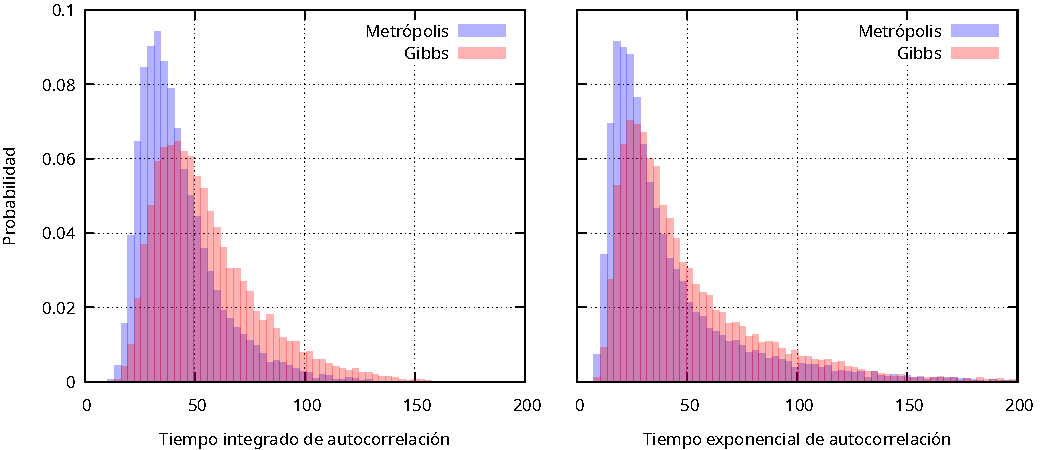
\includegraphics[width = \textwidth]{../img/hist.pdf}
    \caption{Histogramas de $\tauint$ y $\tauexp$ para muestras tomadas con el algoritmo de Metrópolis y Gibbs sampler. Cada histograma se armó con al rededor de 16000 datos tomados de cadenas de Markov que pasaran el test de Gelman-Rubin.}
    \label{fig::hist}
\end{figure}

Dado que cada modelo pasó el test de Gelman-Rubin con $n = 1024$, esperamos que los tiempos de autocorrelación estén muy por debajo de $n$. En otras palabras, si $\tauint$ fuera comparable con $n$, las $n$ muestras usadas para calcular $\hat{R}$ estarían muy correlacionadas, lo que provocaría que el test de Gelman-Rubin falle. En la Figura \ref{fig::hist} vemos que las distribuciones de $\tauint$ presentan picos al rededor de $\tauint = 40$. Podemos interpretar esto como que si tomamos una de cada 80 muestras (una de cada $2\tauint$) y descartamos las demás, ¡Lo que nos queda es una muestra aproximadamente independiente! (aunque 80 veces mas pequeña). Así, al hacer el test de Gelman-Rubin con muestras de tamaño $n = 1024$, entran al rededor de 10 muestras independientes en los cálculos de $\hat{R}$. Cabe notar que Gelman y Rubin recomiendan tomar, al menos, $n \sim 5\tauint$ (ver \cite[Capítulo 11]{gelman2013bayesian}). Por supuesto, uno no puede conocer $\tauint$ antes de haber pasado el burn-in, y no puede saber si ha pasado el burn-in antes de calcular $\hat{R}$, y no puede calcular $\hat{R}$ sin haber elegido $n$. Así, el lector se dará cuenta que, en la práctica, el uno debe explorar un poco hasta decidirse por un valor apropiado de $n$.\\

Antes mencionamos que, como cada dimensión del modelo de Ising puede tomar únicamente dos valores, no esperábamos ver gran diferencia entre el algoritmo de Metrópolis y el Gibbs sampler a la hora de generar muestras. Sin embargo, en la Figura \ref{fig::hist} se ve que el algoritmo de Metrópolis produce muestras ligeramente menos correlacionadas. 

\section{Conclusiones}

Estudiamos e implementamos el test de Gelman-Rubin sobre el modelo de Ising para estimar el tamaño del burn-in de dos métodos de tipo MCMC (el algoritmo de Metrópolis y el Gibbs sampler) usados para muestrear el espacio de estados del modelo. Una vez pasado el burn-in, calculamos $\tauint$ y $\tauexp$. Hemos visto, sin embargo, que no es sencillo elegir los parámetros para poder aplicar estos tests. La elección de parámetros (y, más generalmente, la elección de tests) siempre depende del caso de estudio y el conocimiento a priori que se tenga.\\

Creemos que este trabajo (la sección de motivación, en particular) puede mejorarse agregando un ejemplo de lo que ocurre si no estimamos correctamente el tamaño del burn-in. Por ejemplo, podríamos elegir una temperatura $T$ para la cual el burn-in sea engañosamente largo, calcular un observable del sistema y discutir que los resultados no tienen sentido. Esto fue, en parte, lo que se hizo en el TP 4 de la materia. No lo replicamos en este trabajo por falta de tiempo.\\

En un futuro, sería interesante programar un {\it inicializador dinámico} que pruebe y ajuste los parámetros $m$, $n$ y $N$ a medida que sea necesario. Aunque creemos que es mejor que uno mismo, guiado por su conocimiento a priori de la distribución que desea muestrear, elija estos parámetros manualmente. También nos resulta atractivo reprogramar los modelos y tests usando CUDA (la plataforma de programación paralela de NVIDIA) para aprovechar las capacidades de procesamiento paralelo.

\printbibliography

\end{document}